\newpage
\section{Introduction}

This report will summarize the main points describing the process of making a software product for a Top Trumps game in Java.

It starts off with an outline of the preliminary work required to initiate the work, including the requirements as identified by the team, Spints planning for both the Command Line and Online modes of the game, and also Burndown Charts reflecting the story points as a function of time with expected and actual measurements.

It continues with a section about the assumptions made for the implementation of the product and a chapter summarising the functionality , game logic and database behaviour for both modes.

Details of the testings for each story with corresponding results follow after that, as well as a required section about the current state of the program, under the deficiencies section.

Finally, the appendices contain information about the minutes of meetings (Appendix A), the customer specification defining the requirements (Appendix B), tables with the User Stories with descriptions and acceptance tests (Appendix C), and concludes with supporting screenshots that are referenced throughout the report (Appendix D).

\subsection{A Sample Subheading}

\textbf{This is bold text.}
\emph{This is italic text.}
\todo{A todo example} This is an example of text tagged with a todo item.
Images can be inserted as below, put them into the \emph{img} folder.
If you want a caption (which will automatically be numbered and referenced in the list of figures), include the \emph{captionof} tag as below.

\begin{center}
	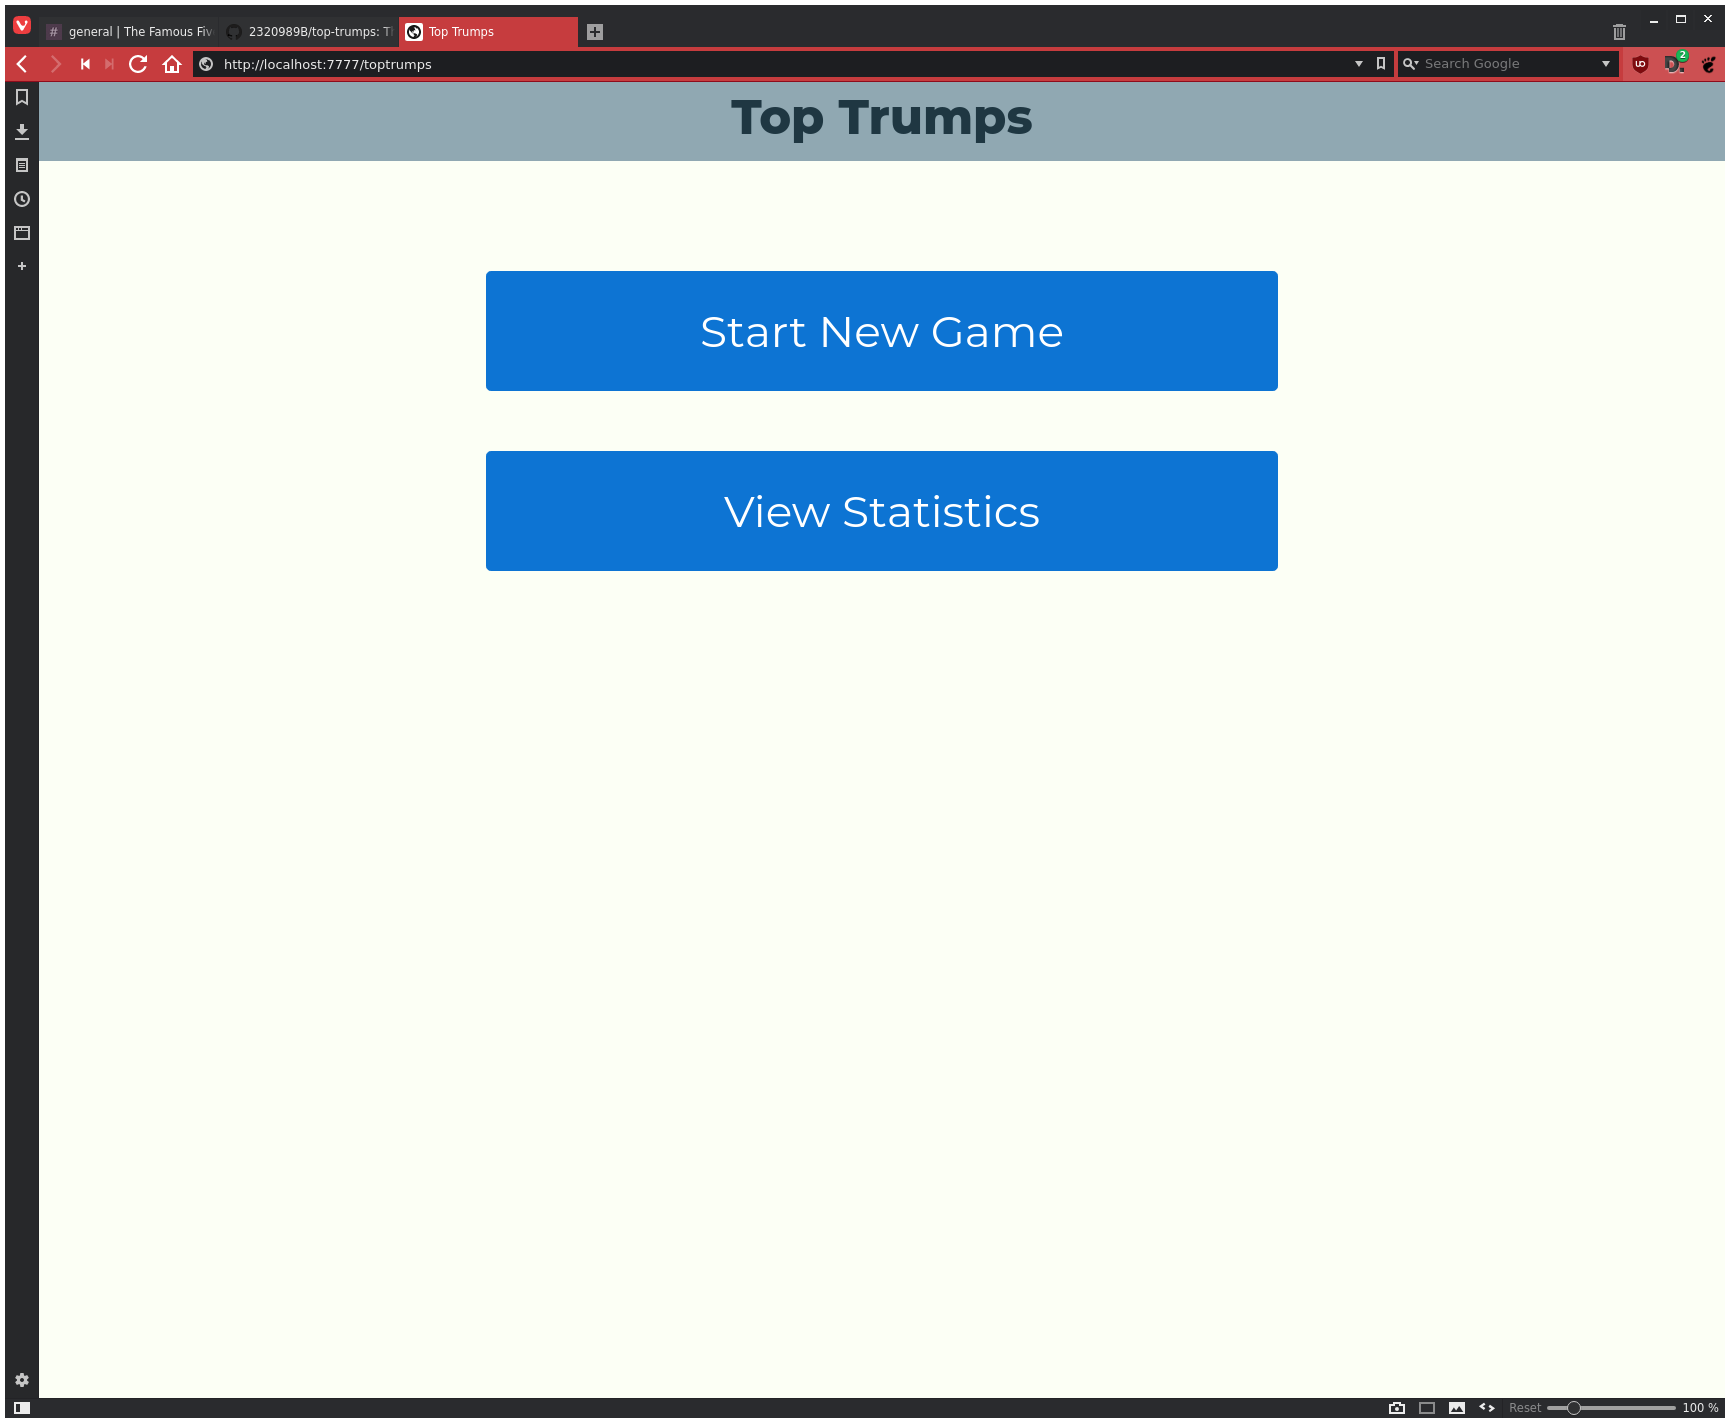
\includegraphics[scale=0.2]{sample.png}
	\captionof{figure}{Main Menu.}
\end{center}